


\begin{frame}{Table of Contents}
   \begin{block}{FLOPs and Bandwidth} \end{block}
   \begin{block}{Performance Modeling} \end{block}
   \begin{block}{PETSc Profiling} \end{block}
   \begin{block}{PETSc and Threads} \end{block}
   \begin{block}{PETSc and GPUs} \end{block}
\end{frame}



%
% FLOPs and Bandwidth
%
\section{FLOPs and Bandwidth}

\section{PETSc Tutorial}
\begin{frame}{PETSc}
   \begin{center} \Large \textbf{FLOPs and Bandwidth} \end{center}
\end{frame}





\begin{frame}{Introduction}
 \vspace*{-0.5cm}
 \begin{center}
  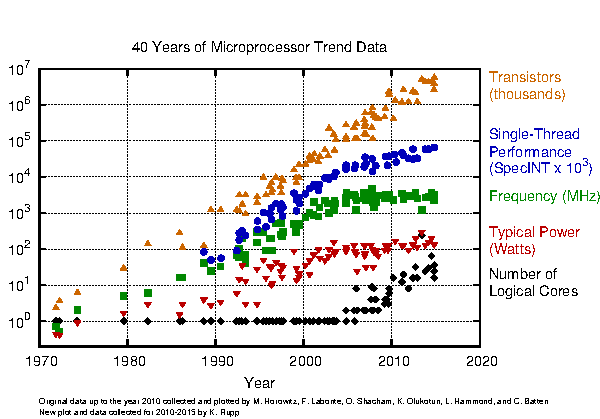
\includegraphics[width=0.95\textwidth]{figures/40-years-processor-trend}
 \end{center}
 {\tiny https://www.karlrupp.net/2015/06/40-years-of-microprocessor-trend-data/ }
\end{frame}

\begin{frame}{Introduction}
 \vspace*{-0.5cm}
 \begin{center}
  Theoretical Peak Performance \\
  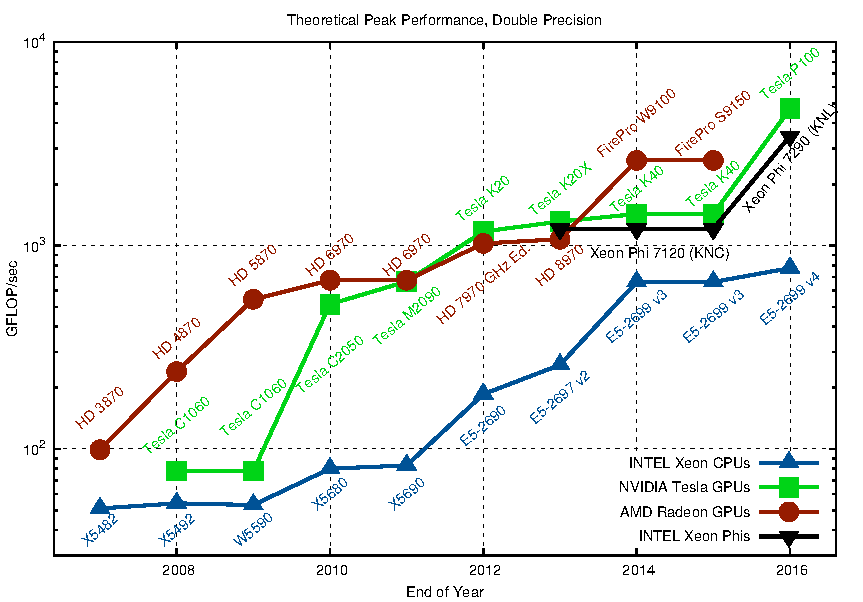
\includegraphics[width=0.95\textwidth]{figures/gflops-dp}
 \end{center}
 \vspace*{-0.5cm}
 {\tiny https://www.karlrupp.net/2013/06/cpu-gpu-and-mic-hardware-characteristics-over-time/ }
\end{frame}

\begin{frame}{Introduction}
 \vspace*{-0.5cm}
 \begin{center}
  Theoretical Peak Performance per Watt \\
  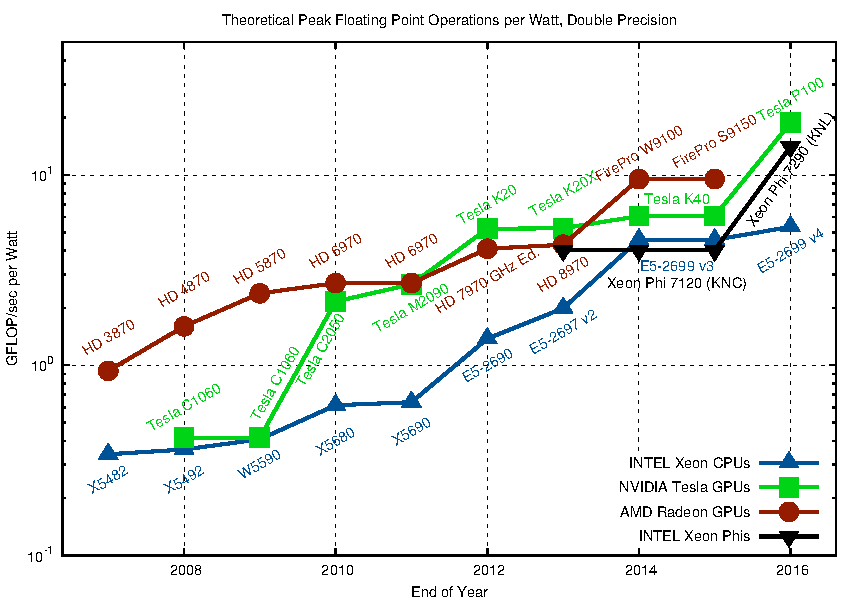
\includegraphics[width=0.95\textwidth]{figures/gflops-per-watt-dp}
 \end{center}
 \vspace*{-0.5cm}
 {\tiny https://www.karlrupp.net/2013/06/cpu-gpu-and-mic-hardware-characteristics-over-time/ }
\end{frame}

\begin{frame}{Introduction}
 \vspace*{-0.5cm}
 \begin{center}
  Memory Bandwidth \\
  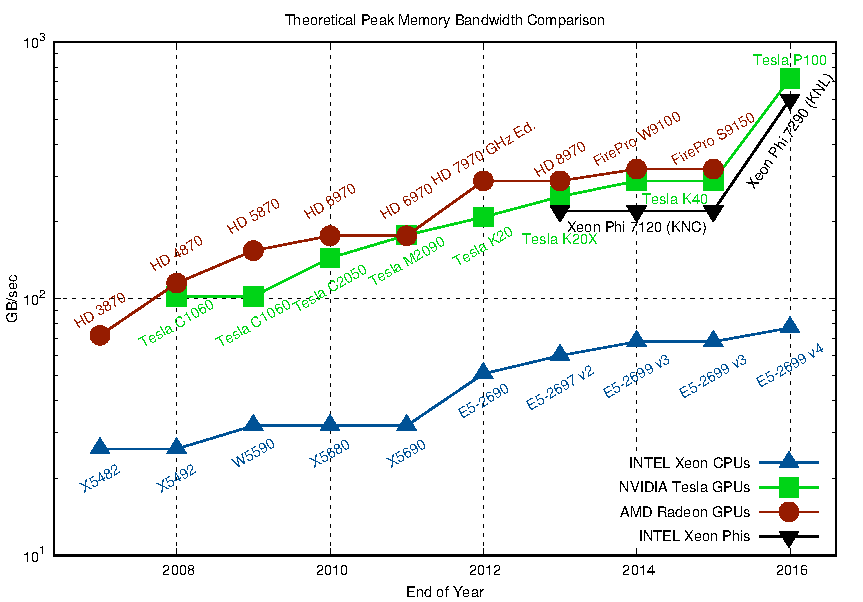
\includegraphics[width=0.95\textwidth]{figures/mem-bw}
 \end{center}
 \vspace*{-0.5cm}
 {\tiny https://www.karlrupp.net/2013/06/cpu-gpu-and-mic-hardware-characteristics-over-time/ }
\end{frame}

\begin{frame}{Introduction}
 \vspace*{-0.5cm}
 \begin{center}
  Theoretical Peak Performance (FLOPs) per Byte of Memory Bandwidth \\
  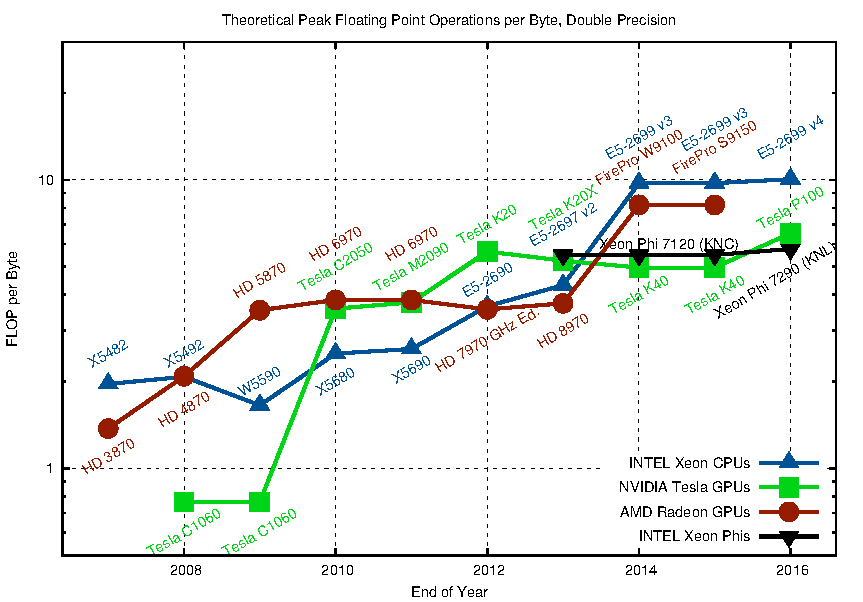
\includegraphics[width=0.95\textwidth]{figures/flop-per-byte-dp}
 \end{center}
 \vspace*{-0.5cm}
 {\tiny https://www.karlrupp.net/2013/06/cpu-gpu-and-mic-hardware-characteristics-over-time/ }
\end{frame}



\begin{frame}[fragile]{FLOPs and Bandwidth}

\  \begin{block}{Typical PETSc Operations}
  \begin{itemize}
   \item Vector operations (add, dot, etc.)
   \item Sparse matrix-vector products (Krylov solvers, smoothers, residuals, etc.)
  \end{itemize}
 \end{block}

 \begin{block}{Maximizing Memory Bandwidth}
  \begin{itemize}
   \item Read contiguous blocks of memory (contiguous access)
   \item Avoid unordered reads whenever possible
  \end{itemize}
 \end{block}

\end{frame}


\begin{frame}[fragile]{FLOPs and Bandwidth}

  \begin{block}{Check Memory Bandwidth Yourself}
  \begin{itemize}
   \item \lstinline|make streams|
   %\pause
   \item Performance question to \verb|petsc-maint|, about 2h ago:
   \begin{lstlisting}
np  speedup
1   1.0
2   1.85
3   2.25
4   2.37
(...)
39  2.47
40  2.45
Estimation of possible speedup of MPI programs based on Streams benchmark.
It appears you have 1 node(s)
    \end{lstlisting}
  \end{itemize}
 \end{block}

\end{frame}

\begin{frame}[fragile]{FLOPs and Bandwidth}

\begin{block}{How does Memory Bandwidth Scale with Cores?}
 \begin{itemize}
  \item Usually saturates quickly
  \item 8-16 processes/threads usually suffice
 \end{itemize}
\end{block}

\begin{center}
 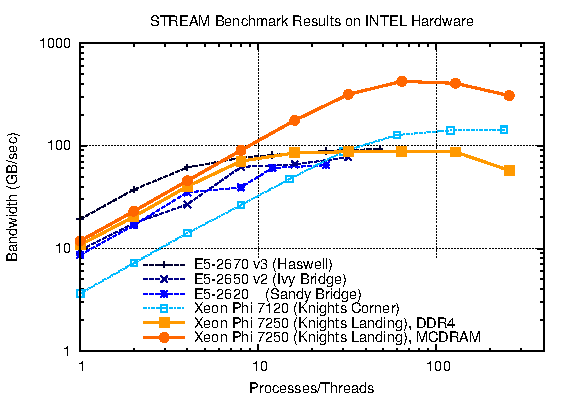
\includegraphics[width=0.7\textwidth]{figures/stream}
\end{center}

\end{frame}



\begin{frame}[fragile]{FLOPs and Bandwidth}

\begin{block}{Offset Memory Access}
  \begin{lstlisting}
void work(double *x, double *y, double *z, int N, int k)
{
  for (size_t i=0; i<N; ++i)
    z[i+k] = x[i+k] + y[i+k];
}  
  \end{lstlisting}
\end{block}

\vspace*{-0.5cm}
\begin{center}
 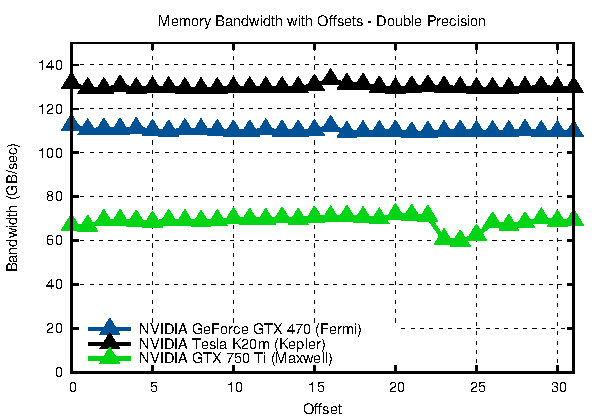
\includegraphics[width=0.6\textwidth]{figures/offset}
\end{center}

\end{frame}




\begin{frame}[fragile]{FLOPs and Bandwidth}

\begin{block}{Strided Memory Access}
  \begin{lstlisting}
void work(double *x, double *y, double *z, int N, int k)
{
  for (size_t i=0; i<N; ++i)
    z[i*k] = x[i*k] + y[i*k];
}  
  \end{lstlisting}
\end{block}

\vspace*{-0.5cm}
\begin{center}
 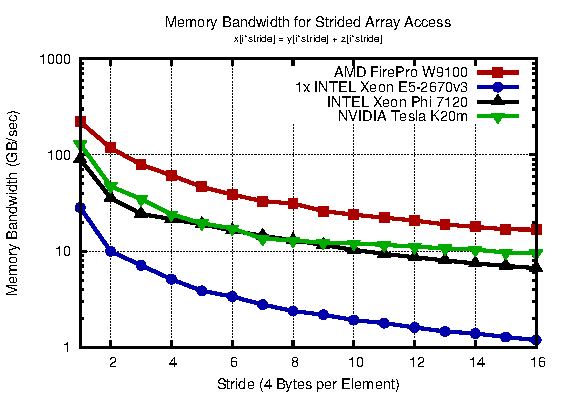
\includegraphics[width=0.6\textwidth]{figures/strided-access}
\end{center}

\end{frame}


%%

\begin{frame}[fragile]{FLOPs and Bandwidth}

\begin{block}{Strided Memory Access}
  \begin{itemize}
   \item Array of structs problematic
  \end{itemize}
  \begin{lstlisting}  
typedef struct particle
{
  double pos_x; double pos_y; double pos_z;
  double vel_x; double vel_y; double vel_z;
  double mass;
} Particle;
  
void increase_mass(Particle *particles, int N)
{
  for (int i=0; i<N; ++i)
    particles[i].mass *= 2.0;
}  
  \end{lstlisting}
\end{block}
   %\pause
   \begin{center} \includegraphics[width=0.7\textwidth]{figures/particles-strided} \end{center}

\end{frame}

%%%

\begin{frame}[fragile]{FLOPs and Bandwidth}

\begin{block}{Strided Memory Access}
  \begin{itemize}
   \item Workaround: Structure of Arrays
  \end{itemize}
  \begin{lstlisting}  
typedef struct particles
{
  double *pos_x; double *pos_y; double *pos_z;
  double *vel_x; double *vel_y; double *vel_z;
  double *mass;
} Particle;
  
void increase_mass(Particle *particles, int N)
{
  for (int i=0; i<N; ++i)
    particles.mass[i] *= 2.0;
}  
  \end{lstlisting}
\end{block}

   %\pause
   \begin{center} 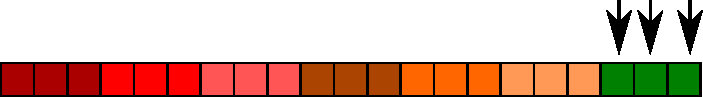
\includegraphics[width=0.7\textwidth]{figures/particles-contiguous} \end{center} \vspace*{0.5cm}

\end{frame}


\begin{frame}{PETSc}
   \begin{center} \Large \textbf{Mindlessly applying object-oriented programming \\[1em]
                                 all the way down to fine granularity \\[1em]
                                 is a recipe for a performance disaster.} \end{center}
                                                                               
\end{frame}



%
% Performance Modeling
%
\section{Performance Modeling}

\section{PETSc Tutorial}
\begin{frame}{PETSc Tutorial}
   \begin{center} \Large \textbf{Performance Modeling} \end{center}
\end{frame}

\begin{frame}{Performance Modeling Mantra}
  \begin{center}
   \LARGE \hspace*{-1cm} \emph{At any given time during a run, \\
                               at least one hardware component\\
                               is operating at 100 percent capacity.}
  \end{center}
\end{frame}


% Latency

\begin{frame}[fragile]{Bottleneck Potpourri}

 \begin{block}{Latency}
  \begin{itemize}
   \item Bottleneck in strong scaling limit
   \item Ultimate limit for time stepping
  \end{itemize}
 \end{block}

 %\pause
 \begin{block}{Latency - Sources}
  \begin{itemize}
   \item Network latency (Ethernet $\sim 20 \mu$s, Infiniband $\sim 5 \mu$s)
   \item PCI-Express latency (Kernel launches, $\sim 10 \mu$s)
   \item Thread synchronization (barriers, locks, $\sim 1-100 \mu$s)
   \item Memory latency ($\sim 100$ns)
  \end{itemize}
 \end{block}

\end{frame}


% Arithmetic intensity: FLOP vs. bandwidth limited
\begin{frame}[fragile]{Bottleneck Potpourri}

 \begin{block}{Arithmetic Intensity}
  \begin{itemize}
   \item Number of FLOPs per Byte
   \item FLOP-limited: Arithmetic intensity larger than $\sim$10
   \item Memory-limited: Arithmetic intensity smaller than $\sim$1
  \end{itemize}
 \end{block}

 \vspace*{-0.5cm}
 \begin{center}
   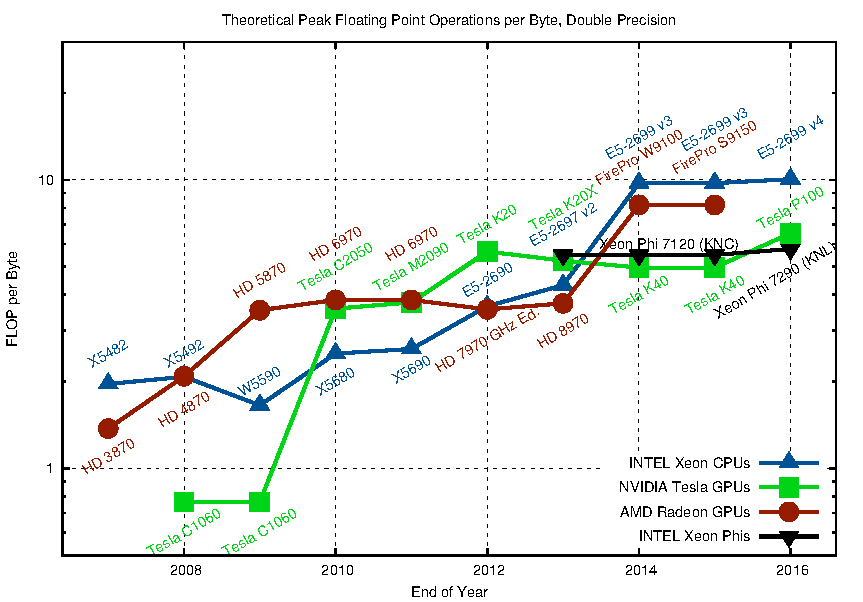
\includegraphics[width=0.7\textwidth]{figures/flop-per-byte-dp}
 \end{center}

\end{frame}






%% 12. Modeling by Example


\begin{frame}{Performance Modeling: Vector Addition}

 \begin{block}{Vector Addition}
  \begin{itemize}
   \item $x = y + z$ with $N$ elements each
   \item 1 FLOP per 24 byte in double precision
   \item Limited by memory bandwidth $\Rightarrow T_2(N) \stackrel{?}{\approx} 3 \times 8 \times N / \mathrm{Bandwidth} + \mathrm{Latency}$
  \end{itemize}
 \end{block}

 \vspace*{-0.5cm}
 \begin{center}
  \only<1>{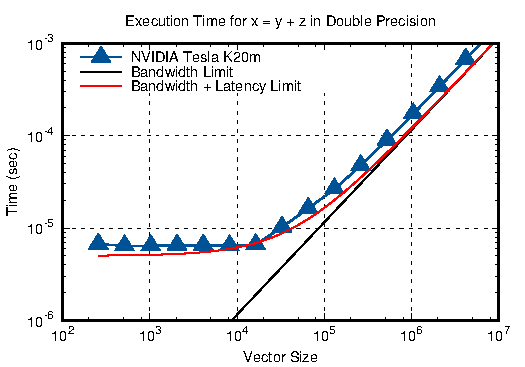
\includegraphics[width=0.75\textwidth]{figures/vector-addition-time-3}}
  
  \only<2>{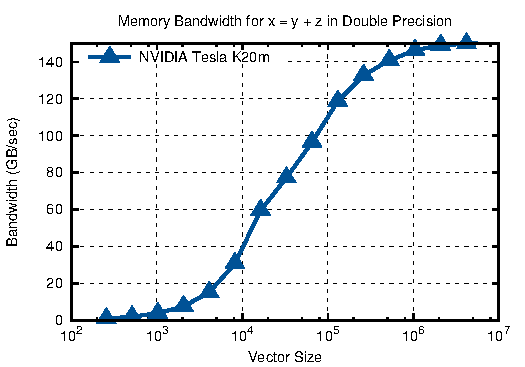
\includegraphics[width=0.75\textwidth]{figures/vector-addition-bw}}
 \end{center}
 
 \end{frame}








%
% Debugging and Profiling
%
\section{PETSc Profiling}
\begin{frame}{PETSc Tutorial}
   \begin{center} \Large \textbf{PETSc Profiling} \end{center}
\end{frame}

\begin{frame}[fragile]{PETSc Profiling}

\begin{block}{First: Get the Math Right!}
\begin{itemize}
  \item Choose an algorithm that gives robust iteration counts
  \item Choose an algorithm that really converges
\end{itemize}  
\end{block}
  
%\pause
\begin{block}{Profiling}
\begin{itemize}
  \item Use \lstinline|-log_view| for a performance profile
  \begin{itemize}
    \item Event timing
    \item Event flops
    \item Memory usage
    \item MPI messages
  \end{itemize}

  \item Call \lstinline|PetscLogStagePush()| and \lstinline|PetscLogStagePop()|
  \begin{itemize}
    \item User can add new stages
  \end{itemize}

  \item Call \lstinline|PetscLogEventBegin()| and \lstinline|PetscLogEventEnd()|
  \begin{itemize}
    \item User can add new events
  \end{itemize}

  \item Call \lstinline|PetscLogFlops()| to include your flops
\end{itemize}
\end{block}

\end{frame}

\begin{frame}[fragile]{PETSc Profiling}

\begin{block}{Reading -log\_summary}
\begin{itemize}
\item
{\scriptsize
\begin{verbatim}
                         Max       Max/Min        Avg      Total 
Time (sec):           1.548e+02      1.00122   1.547e+02
Objects:              1.028e+03      1.00000   1.028e+03
Flops:                1.519e+10      1.01953   1.505e+10  1.204e+11
Flops/sec:            9.814e+07      1.01829   9.727e+07  7.782e+08
MPI Messages:         8.854e+03      1.00556   8.819e+03  7.055e+04
MPI Message Lengths:  1.936e+08      1.00950   2.185e+04  1.541e+09
MPI Reductions:       2.799e+03      1.00000
\end{verbatim}}
\item Also a summary per stage
\item Memory usage per stage (based on when it was allocated)
\item Time, messages, reductions, balance, flops per event per stage
\item Always send \lstinline|-log_summary| when asking \\
  performance questions on mailing list
\end{itemize}
\end{block}
\end{frame}

\begin{frame}[fragile]{PETSc Profiling}

%[basicstyle=\tiny\ttfamily]
{ \tiny
\begin{verbatim}
Event                Count      Time (sec)     Flops                             --- Global ---  --- Stage ---   Total
                   Max Ratio  Max     Ratio   Max  Ratio  Mess   Avg len Reduct  %T %F %M %L %R  %T %F %M %L %R Mflop/s
------------------------------------------------------------------------------------------------------------------------
--- Event Stage 1: Full solve
VecDot                43 1.0 4.8879e-02 8.3 1.77e+06 1.0 0.0e+00 0.0e+00 4.3e+01  0  0  0  0  0   0  0  0  0  1 73954
VecMDot             1747 1.0 1.3021e+00 4.6 8.16e+07 1.0 0.0e+00 0.0e+00 1.7e+03  0  1  0  0 14   1  1  0  0 27 128346
VecNorm             3972 1.0 1.5460e+00 2.5 8.48e+07 1.0 0.0e+00 0.0e+00 4.0e+03  0  1  0  0 31   1  1  0  0 61 112366
VecScale            3261 1.0 1.6703e-01 1.0 3.38e+07 1.0 0.0e+00 0.0e+00 0.0e+00  0  0  0  0  0   0  0  0  0  0 414021
VecScatterBegin     4503 1.0 4.0440e-01 1.0 0.00e+00 0.0 6.1e+07 2.0e+03 0.0e+00  0  0 50 26  0   0  0 96 53  0     0
VecScatterEnd       4503 1.0 2.8207e+00 6.4 0.00e+00 0.0 0.0e+00 0.0e+00 0.0e+00  0  0  0  0  0   0  0  0  0  0     0
MatMult             3001 1.0 3.2634e+01 1.1 3.68e+09 1.1 4.9e+07 2.3e+03 0.0e+00 11 22 40 24  0  22 44 78 49  0 220314
MatMultAdd           604 1.0 6.0195e-01 1.0 5.66e+07 1.0 3.7e+06 1.3e+02 0.0e+00  0  0  3  0  0   0  1  6  0  0 192658
MatMultTranspose     676 1.0 1.3220e+00 1.6 6.50e+07 1.0 4.2e+06 1.4e+02 0.0e+00  0  0  3  0  0   1  1  7  0  0 100638
MatSolve            3020 1.0 2.5957e+01 1.0 3.25e+09 1.0 0.0e+00 0.0e+00 0.0e+00  9 21  0  0  0  18 41  0  0  0 256792
MatCholFctrSym         3 1.0 2.8324e-04 1.0 0.00e+00 0.0 0.0e+00 0.0e+00 0.0e+00  0  0  0  0  0   0  0  0  0  0     0
MatCholFctrNum        69 1.0 5.7241e+00 1.0 6.75e+08 1.0 0.0e+00 0.0e+00 0.0e+00  2  4  0  0  0   4  9  0  0  0 241671
MatAssemblyBegin     119 1.0 2.8250e+00 1.5 0.00e+00 0.0 2.1e+06 5.4e+04 3.1e+02  1  0  2 24  2   2  0  3 47  5     0
MatAssemblyEnd       119 1.0 1.9689e+00 1.4 0.00e+00 0.0 2.8e+05 1.3e+03 6.8e+01  1  0  0  0  1   1  0  0  0  1     0
SNESSolve              4 1.0 1.4302e+02 1.0 8.11e+09 1.0 6.3e+07 3.8e+03 6.3e+03 51 50 52 50 50  99100 99100 97 113626
SNESLineSearch        43 1.0 1.5116e+01 1.0 1.05e+08 1.1 2.4e+06 3.6e+03 1.8e+02  5  1  2  2  1  10  1  4  4  3 13592
SNESFunctionEval      55 1.0 1.4930e+01 1.0 0.00e+00 0.0 1.8e+06 3.3e+03 8.0e+00  5  0  1  1  0  10  0  3  3  0     0
SNESJacobianEval      43 1.0 3.7077e+01 1.0 7.77e+06 1.0 4.3e+06 2.6e+04 3.0e+02 13  0  4 24  2  26  0  7 48  5   429
KSPGMRESOrthog      1747 1.0 1.5737e+00 2.9 1.63e+08 1.0 0.0e+00 0.0e+00 1.7e+03  1  1  0  0 14   1  2  0  0 27 212399
KSPSetup             224 1.0 2.1040e-02 1.0 0.00e+00 0.0 0.0e+00 0.0e+00 3.0e+01  0  0  0  0  0   0  0  0  0  0     0
KSPSolve              43 1.0 8.9988e+01 1.0 7.99e+09 1.0 5.6e+07 2.0e+03 5.8e+03 32 49 46 24 46  62 99 88 48 88 178078
PCSetUp              112 1.0 1.7354e+01 1.0 6.75e+08 1.0 0.0e+00 0.0e+00 8.7e+01  6  4  0  0  1  12  9  0  0  1 79715
PCSetUpOnBlocks     1208 1.0 5.8182e+00 1.0 6.75e+08 1.0 0.0e+00 0.0e+00 8.7e+01  2  4  0  0  1   4  9  0  0  1 237761
PCApply              276 1.0 7.1497e+01 1.0 7.14e+09 1.0 5.2e+07 1.8e+03 5.1e+03 25 44 42 20 41  49 88 81 39 79 200691
\end{verbatim}
}
\end{frame}

\begin{frame}{PETSc Profiling}

\begin{block}{Communication Costs}
  \begin{itemize}
  \item Reductions: usually part of Krylov method, latency limited
    \begin{itemize}
    \item \lstinline|VecDot|
    \item \lstinline|VecMDot|
    \item \lstinline|VecNorm|
    \item \lstinline|MatAssemblyBegin|
    \item Change algorithm (e.g. IBCGS)
    \end{itemize}
  \item Point-to-point (nearest neighbor), latency or bandwidth
    \begin{itemize}
    \item \lstinline|VecScatter|
    \item \lstinline|MatMult|
    \item \lstinline|PCApply|
    \item \lstinline|MatAssembly|
    \item \lstinline|SNESFunctionEval|
    \item \lstinline|SNESJacobianEval|
    \item Compute subdomain boundary fluxes redundantly
    \item Ghost exchange for all fields at once
    \item Better partition
    \end{itemize}
  \end{itemize}
  \end{block}
\end{frame}



\begin{frame}[fragile]{PETSc Profiling}

  \begin{block}{Adding a Logging Event (C)}
   \begin{lstlisting}
 PetscLogEvent  USER_EVENT;
 PetscClassId   classid;
 PetscLogDouble user_event_flops;
 
 PetscClassIdRegister("class name",&classid);
 PetscLogEventRegister("user event",classid,&USER_EVENT);
 
 PetscLogEventBegin(USER_EVENT,0,0,0,0);
    /* code segment to monitor */
 PetscLogFlops(user_event_flops);
 PetscLogEventEnd(USER_EVENT,0,0,0,0);
\end{lstlisting}
  \end{block}

  \begin{block}{Adding a Logging Event (Python)}
   \begin{lstlisting}
with PETSc.logEvent('Reconstruction') as recEvent:
    # All operations are timed in recEvent
    reconstruct(sol)
    # Flops are logged to recEvent
    PETSc.Log.logFlops(user_event_flops)
\end{lstlisting}
  \end{block}

\end{frame}


\begin{frame}[fragile]{PETSc Profiling}

  \begin{block}{Adding a Logging Stage (C)}
   \begin{lstlisting}
PetscLogStage stage;

PetscLogStageRegister("name", &stage);
PetscLogStagePush(stage);

/* Code to Monitor */

PetscLogStagePop();
\end{lstlisting}
  \end{block}

\end{frame}


\begin{frame}[fragile]{PETSc Profiling}

%[basicstyle=\tiny\ttfamily]
{ \tiny
\begin{verbatim}
Event                  Count      Time (sec)     Flops                             --- Global ---  --- Stage ---   Total
                     Max Ratio  Max     Ratio   Max  Ratio  Mess   Avg len Reduct  %T %F %M %L %R  %T %F %M %L %R Mflop/s
------------------------------------------------------------------------------------------------------------------------
--- Event Stage 0: Main Stage

MatMult              178 1.0 7.8040e+01 1.0 2.59e+11 1.0 4.4e+02 2.0e+05 0.0e+00   33 41  6 11  0  51 89 20 24  0  6648
MatPtAP               10 1.0 2.4870e+01 1.0 5.45e+09 1.0 2.1e+02 3.1e+05 1.8e+02   10  1  3  8  1  16  2  9 18  4   429
MatPtAPSymbolic       10 1.0 1.8828e+01 1.0 0.00e+00 0.0 1.2e+02 2.7e+05 8.2e+01    8  0  2  4  0  12  0  5  9  2     0
MatPtAPNumeric        10 1.0 6.0428e+00 1.0 5.45e+09 1.0 9.4e+01 3.7e+05 1.0e+02    3  1  1  4  0   4  2  4  9  2  1767
SNESSolve              2 1.0 1.9059e+02 1.0 6.22e+11 1.0 6.6e+03 9.3e+04 3.4e+03   79 99 92 75 16 123213292168 83  6509
KSPSolve               2 1.0 1.8230e+02 1.0 6.07e+11 1.0 6.5e+03 9.1e+04 3.2e+03   76 97 89 72 15 118208285161 77  6647
PCSetUp                8 1.0 1.6138e+01 1.0 4.81e+09 1.1 1.2e+03 8.1e+04 2.5e+03    7  1 17 12 11  10  2 55 28 60   582
PCApply               46 1.0 1.2586e+02 1.0 4.43e+11 1.0 6.3e+03 8.5e+04 2.7e+03   52 70 87 65 12  81152277146 64  7022
KSPSolve_FS_0         46 1.0 1.0038e+02 1.0 3.42e+11 1.0 6.2e+03 8.2e+04 2.6e+03   42 54 86 62 12  65117273138 64  6792
(...)

--- Event Stage 1: MG Apply

MatMultMFA11         296 1.0 4.3461e+01 1.0 2.82e+11 1.0 1.2e+03 3.0e+05 0.0e+00   18 45 16 43  0  51 84 24 78  0 12995
KSPSolve             230 1.0 7.2581e+01 1.0 2.87e+11 1.0 4.5e+03 8.5e+04 2.6e+02   30 46 62 47  1  85 85 91 84100  7872
PCApply              642 1.0 1.0269e+01 1.0 1.40e+10 1.1 3.0e+03 8.7e+03 1.8e+02    4  2 42  3  1  12  4 61  6 68  2645
MGSmooth Level 0      46 1.0 7.8169e+00 1.0 1.06e+10 1.1 3.0e+03 8.3e+03 1.7e+02    3  2 41  3  1   9  3 61  5 65  2621
MGSmooth Level 1      92 1.0 2.4177e+01 1.0 3.17e+10 1.0 5.0e+02 1.2e+05 4.6e+01   10  5  7  7  0  28  9 10 13 18  2569
MGResid Level 1       46 1.0 4.3231e+00 1.0 5.77e+09 1.0 9.2e+01 1.2e+05 0.0e+00    2  1  1  1  0   5  2  2  2  0  2615
MGInterp Level 1      92 1.0 3.5063e-01 1.1 1.09e+08 1.0 9.2e+01 1.5e+04 0.0e+00    0  0  1  0  0   0  0  2  0  0   612
MGSmooth Level 2      92 1.0 4.0886e+01 1.0 2.44e+11 1.0 1.0e+03 3.0e+05 4.6e+01   17 39 14 37  0  48 73 20 66 18 11954
MGResid Level 2       46 1.0 6.8277e+00 1.0 4.39e+10 1.0 1.8e+02 3.0e+05 0.0e+00    3  7  3  7  0   8 13  4 12  0 12874
MGInterp Level 2      92 1.0 1.0898e+00 1.4 8.47e+08 1.0 9.2e+01 3.8e+04 0.0e+00    0  0  1  0  0   1  0  2  1  0  1544
(...)
------------------------------------------------------------------------------------------------------------------------
\end{verbatim}
}
\end{frame}





%
% Threads
%
\section{PETSc and Threads}

\section{PETSc Tutorial}
\begin{frame}{PETSc Tutorial}
   \begin{center} \Large \textbf{PETSc and Threads} \end{center}
\end{frame}


\begin{frame}[fragile]{PETSc and Threads}

 \begin{block}{Competing Threading Approaches}
  \begin{itemize}
   \item pthread
   \item OpenMP
   \item C++11 threads
   \item Compiler magic
  \end{itemize}
 \end{block}

 %\pause
 \begin{block}{Issues with Threads}
  \begin{itemize}
   \item Problematic across compilers
   \item Data locality
   \item Thread ownership
   \item Software interface
  \end{itemize}
 \end{block}

 %\pause
  \begin{block}{Assumption for Subsequent Discussion}
  \begin{itemize}
   \item Primary Goal: Get the science done!
   \item 10 percent performance difference is \textbf{not significant}
  \end{itemize}
 \end{block}

\end{frame}


\begin{frame}[fragile]{PETSc and Threads}
  \begin{block}{When to Use Threads After All?}
    \begin{itemize}
     \item Distributed Memory: Need MPI anyway
     %\pause
     \item Shared Memory: MPI for multi-socket systems for NUMA reasons
     %\pause
     \item 1-Socket Machines: If a 2-5x gain is critical, use a cluster!
    \end{itemize}
  \end{block}

  \begin{center}
    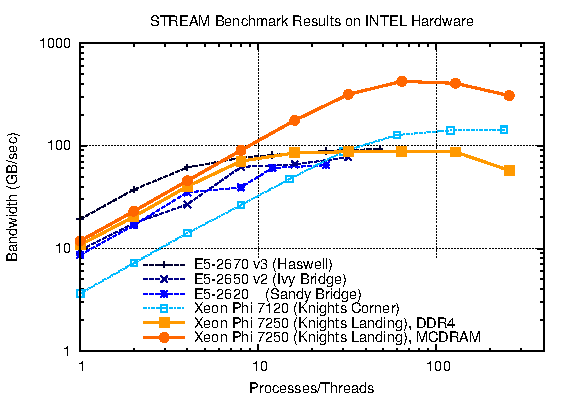
\includegraphics[width=0.55\textwidth]{figures/stream}
  \end{center}
  
\end{frame}


\begin{frame}[fragile]{Threads and Library Interfaces}

 \begin{block}{Attempt 1}
  \begin{itemize}
   \item Library spawns threads
  \end{itemize}
 \end{block}

   \begin{lstlisting}
  void library_func(double *x, int N) {
    #pragma omp parallel for
    for (int i=0; i<N; ++i) x[i] = something_complicated();
  }
  \end{lstlisting}

  %\pause
  
  \begin{block}{Problems}
   \begin{itemize}
    \item Call from multi-threaded environment?
   \begin{lstlisting}
  void user_func(double **y, int N) {
    #pragma omp parallel for
    for (int j=0; j<M; ++j) library_func(y[j], N);
  }
  \end{lstlisting}
    \item Incompatible OpenMP runtimes (e.g. GCC vs. ICC)
   \end{itemize}
 \end{block}

\end{frame}

\begin{frame}[fragile]{Threads and Library Interfaces}

 \begin{block}{Attempt 2}
  \begin{itemize}
   \item Use pthreads/TBB/etc. instead of OpenMP to spawn threads
   \item Fixes incompatible OpenMP implementations (probably)
  \end{itemize}
 \end{block}

  %\pause
  \begin{block}{Problems}
   \begin{itemize}
    \item Still a problem with multi-threaded user environments
   \begin{lstlisting}
  void user_func(double **y, int N) {
    #pragma omp parallel for
    for (int j=0; j<M; ++j) library_func(y[j], N);
  }
   \end{lstlisting}
  \end{itemize}
 \end{block}

\end{frame}


\begin{frame}[fragile]{Threads and Library Interfaces}

 \begin{block}{Attempt 3}
  \begin{itemize}
   \item Hand back thread management to user
  \end{itemize}
 \end{block}

  \begin{lstlisting}
  void library_func(ThreadInfo ti, double *x, int N) {
    int start = compute_start_index(ti, N);
    int stop  = compute_stop_index(ti, N);
    for (int i=start; i<stop; ++i)
      x[i] = something_complicated();
  }
  \end{lstlisting}

  %\pause
  \begin{block}{Implications}
   \begin{itemize}
    \item Users can use their favorite threading model
    \item API requires one extra parameter
    \item Extra boilerplate code required in user code
  \end{itemize}
 \end{block}
\end{frame}


\begin{frame}[fragile]{Threads and Library Interfaces}

 \begin{block}{Reflection}
  \begin{itemize}
   \item Extra thread communication parameter
    \begin{lstlisting}
void library_func(ThreadInfo ti, double *x, int N) {...}
    \end{lstlisting}
    %\pause
   \item Rename thread management parameter
    \begin{lstlisting}
void library_func(Thread_Comm c, double *x, int N) {...}
    \end{lstlisting}
    %\pause
   \item Compare:
    \begin{lstlisting}
void library_func(MPI_Comm comm, double *x, int N) {...}
    \end{lstlisting}
  \end{itemize}
 \end{block}

 %\pause
  \begin{block}{Conclusion}
   \begin{itemize}
    \item Prefer flat MPI over MPI+OpenMP for a composable software stack
    \item MPI automatically brings better data locality
  \end{itemize}
 \end{block}

\end{frame}




%
% GPU Summary
%
\section{PETSc and GPUs}
\begin{frame}{PETSc}
   \begin{center} \Large \textbf{PETSc and GPUs} \end{center}
\end{frame}




% \begin{frame}{Why bother?}
%   \begin{center} \vspace*{-0.5cm}
%    \includegraphics[width=0.9\textwidth]{figures/cuda-advantage-2}
%   \end{center}
% \end{frame}
% 
% \begin{frame}{Why bother?}
%   \begin{center} \vspace*{-0.3cm}
%    \includegraphics[width=0.6\textwidth]{figures/cuda-advantage} \\
%    \visible<2->{
%    
\includegraphics[width=0.6\textwidth]{figures/xkcd-someone-wrong}
%    }
%   \end{center}
% \end{frame}


\begin{frame}{Why bother?}
  \begin{center}
   \LARGE \hspace*{-1cm} \emph{Don't believe anything \\ \hspace*{1cm}unless you can run it}
  \end{center}
  \hspace*{6cm}Matt Knepley
\end{frame}



\begin{frame}{Why bother?}
  \begin{block}{GFLOPs/Watt}
  \begin{center} \vspace*{-0.5cm}
   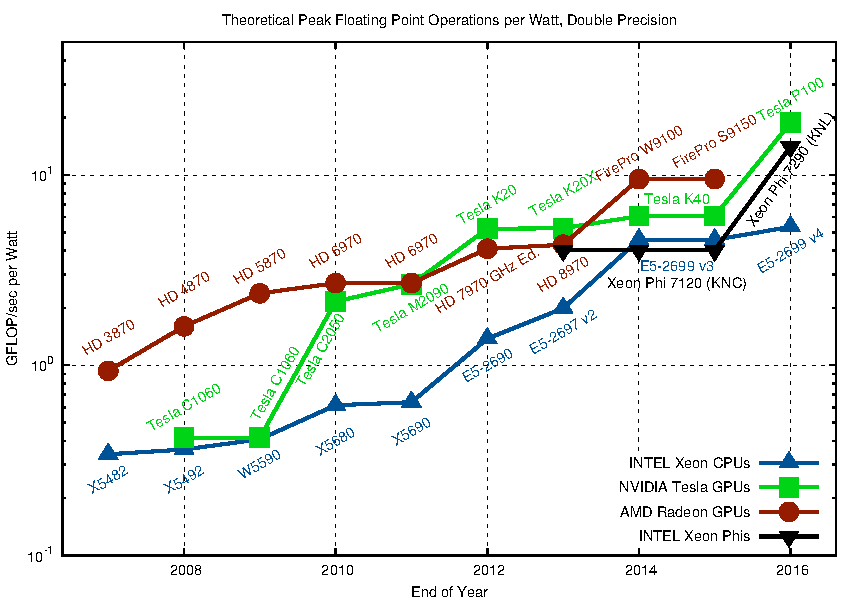
\includegraphics[width=0.95\textwidth]{figures/gflops-per-watt-dp.pdf}
  \end{center}
  \end{block}
\end{frame}



\begin{frame}{Why bother?}
  \begin{block}{Procurements}
  \begin{itemize}
   \item Theta (ANL, 2016): 2nd generation INTEL Xeon Phi
   \item Summit (ORNL, 2017), Sierra (LLNL, 2017): NVIDIA Volta GPU
   \item Aurora (ANL, 2018): 3rd generation INTEL Xeon Phi
  \end{itemize}
  \end{block}
  
  \begin{center} \vspace*{-0.5cm}
   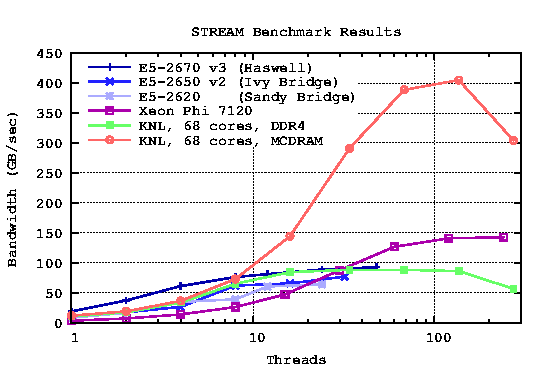
\includegraphics[width=0.75\textwidth]{figures/stream-knl.pdf} \\
   {\tiny https://www.karlrupp.net/2016/07/knights-landing-vs-knights-corner-haswell-ivy-bridge-and-sandy-bridge-stream-benchmark-results/}
  \end{center}

\end{frame}


%%%%%%%%%%%%%%%%%%%%%%%%%%%%%%%%%%%%%%%%%



\begin{frame}{Current Status}
  \begin{center}
    \Large PETSc on GPUs and MIC: \\[1em] Current Status
  \end{center}
\end{frame}

\begin{frame}[fragile]
\frametitle{Available Options}

 \begin{minipage}{0.75\textwidth}
  \begin{block}{Native on Xeon Phi}
  \begin{itemize}
   \item Cross-compile for Xeon Phi
  \end{itemize}
  \end{block}

  \begin{block}{CUDA}
  \begin{itemize}
   \item CUDA-support through CUSP as well as native
   \item \lstinline|-vec_type cusp -mat_type aijcusp|
   \item \lstinline|-vec_type cuda -mat_type aijcusparse|
   \item Only for NVIDIA GPUs
  \end{itemize}
  \end{block}

  \begin{block}{CUDA/OpenCL/OpenMP}
  \begin{itemize}
   \item CUDA/OpenCL/OpenMP-support through ViennaCL
   \item \lstinline|-vec_type viennacl -mat_type aijviennacl|
   \item OpenCL on CPUs and MIC fairly poor
  \end{itemize}
  \end{block}
 \end{minipage}
 \begin{minipage}{0.23\textwidth}
 \vspace*{1cm}
 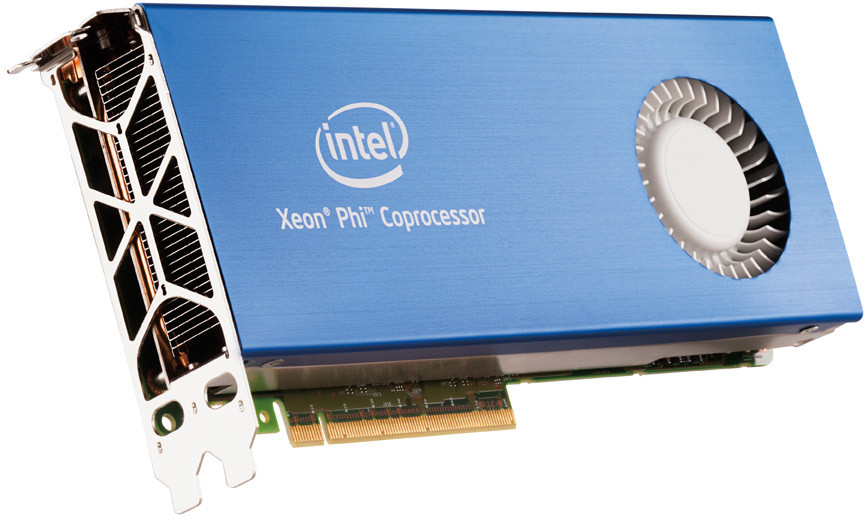
\includegraphics[width=0.99\textwidth]{figures/xeon-phi.jpg} \\[1.5em]
 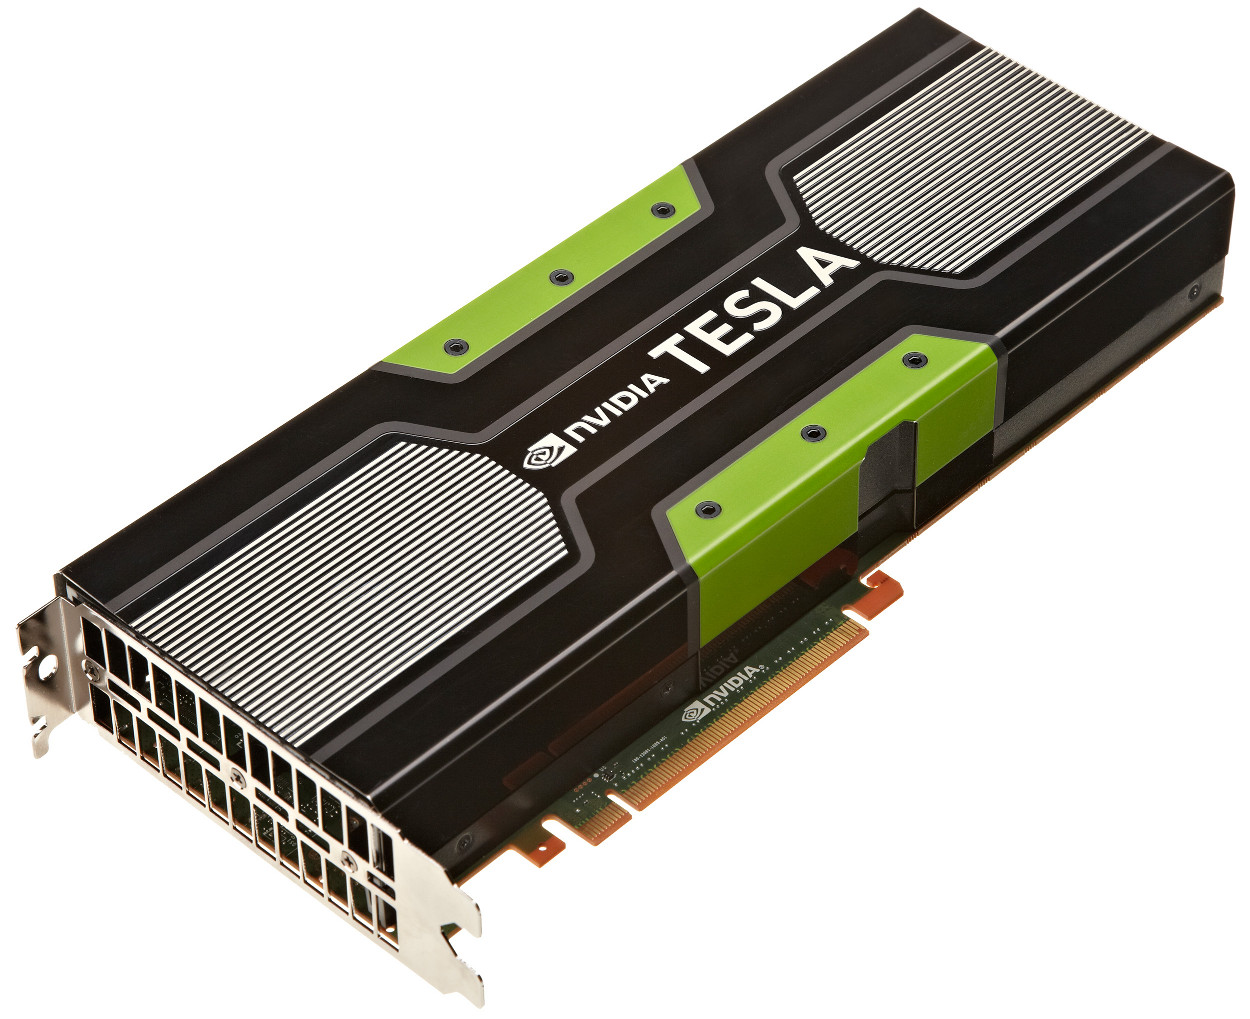
\includegraphics[width=0.99\textwidth]{figures/TeslaK20.jpg} \\[1.5em]
 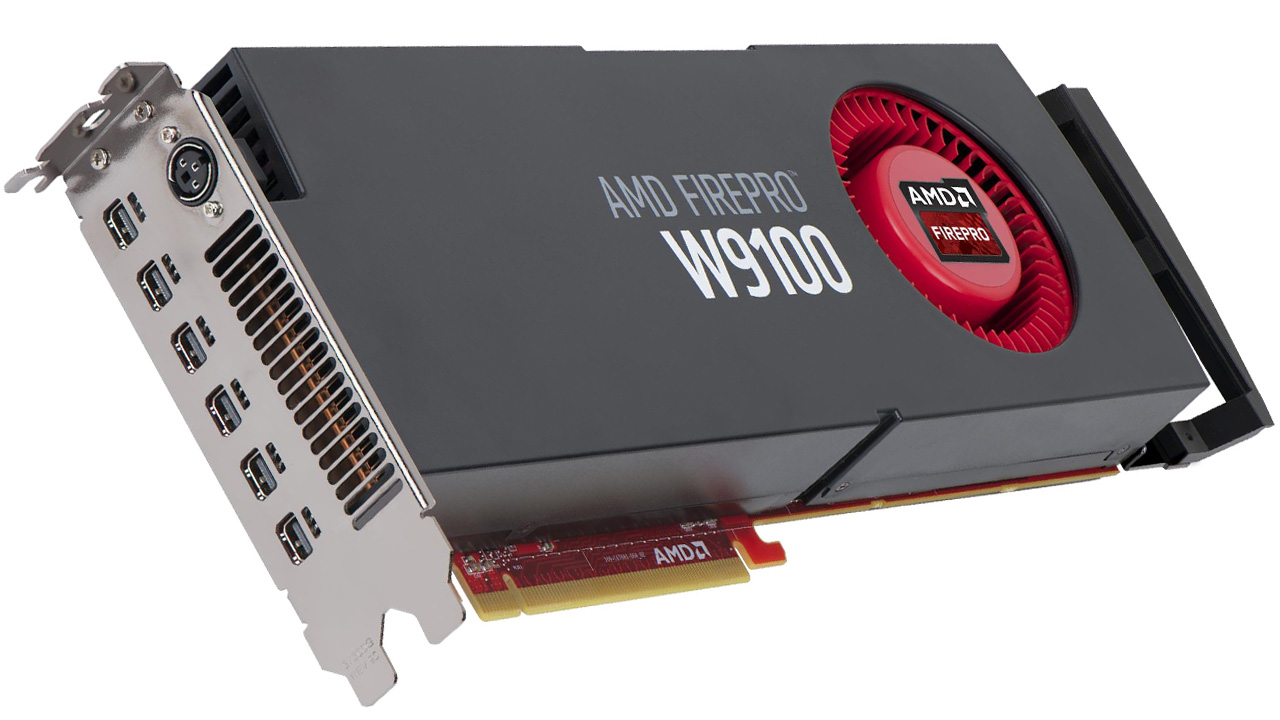
\includegraphics[width=0.99\textwidth]{figures/w9100.jpg} \\[1.5em]
 \end{minipage}


\end{frame}


% Configure PETSc
\begin{frame}[fragile]
\frametitle{Configuration}
  \begin{block}{CUDA}
    \begin{itemize}
     \item CUDA-enabled configuration (minimum)
     \begin{lstlisting}
 ./configure [..] --with-cuda=1
     \end{lstlisting}
     \item With CUSP:
     \begin{lstlisting}
   --with-cusp=1 --with-cusp-dir=/path/to/cusp
     \end{lstlisting}
     \item Customization:
     \begin{lstlisting}
   --with-cudac=/path/to/cuda/bin/nvcc
   --with-cuda-arch=sm_20
     \end{lstlisting}
    \end{itemize}
  \end{block}
  
  \begin{block}{OpenCL (ViennaCL)}
    \begin{itemize}
     \item OpenCL-enabled configuration
     \begin{lstlisting}
 ./configure [..] --download-viennacl
    --with-opencl-include=/path/to/OpenCL/include
    --with-opencl-lib=/path/to/libOpenCL.so
     \end{lstlisting}
    \end{itemize}
  \end{block}
\end{frame}


% How does it work?
\begin{frame}[fragile]
\frametitle{How Does It Work?}
  \begin{block}{Host and Device Data}
  \begin{lstlisting}
struct _p_Vec {
  ...
  void          *data;            // host buffer
  PetscCUSPFlag valid_GPU_array;  // flag
  void          *spptr;           // device buffer
};
  \end{lstlisting}
  \end{block}

  \begin{block}{Possible Flag States}
  \begin{lstlisting}
  typedef enum {PETSC_CUSP_UNALLOCATED,
                PETSC_CUSP_GPU,
                PETSC_CUSP_CPU,
                PETSC_CUSP_BOTH} PetscCUSPFlag;
  \end{lstlisting}
  \end{block}

\end{frame}

\begin{frame}[fragile]
\frametitle{How Does It Work?}

  \begin{block}{Fallback-Operations on Host}
   \begin{itemize}
    \item Data becomes valid on host (\lstinline|PETSC_CUSP_CPU|)
      \begin{lstlisting}
PetscErrorCode VecSetRandom_SeqCUSP_Private(..) {
  VecGetArray(...);
  // some operation on host memory
  VecRestoreArray(...);
}
      \end{lstlisting}
   \end{itemize}
  \end{block}

  %\pause 
  
  \begin{block}{Accelerated Operations on Device}
   \begin{itemize}
    \item Data becomes valid on device (\lstinline|PETSC_CUSP_GPU|)
      \begin{lstlisting}
PetscErrorCode VecAYPX_SeqCUSP(..) {
  VecCUSPGetArrayReadWrite(...);
  // some operation on raw handles on device
  VecCUSPRestoreArrayReadWrite(...);
}
      \end{lstlisting}
   \end{itemize}
  \end{block}

\end{frame}


% Example with ILU
\begin{frame}[fragile]
\frametitle{Example}
  \begin{block}{KSP ex12 on Host}
  \begin{itemize}
   \item
    \begin{lstlisting}
$> ./ex12
    -pc_type ilu -m 200 -n 200 -log_summary
    \end{lstlisting}
    \begin{lstlisting}
KSPGMRESOrthog       228 1.0 6.2901e-01
KSPSolve               1 1.0 2.7332e+00
    \end{lstlisting}

  \end{itemize}
  \end{block}

  %\pause
  
  \begin{block}{KSP ex12 on Device}
  \begin{itemize}
   \item
    \begin{lstlisting}
$> ./ex12 -vec_type cusp -mat_type aijcusp
    -pc_type ilu -m 200 -n 200 -log_summary
    \end{lstlisting}
    \begin{lstlisting}
[0]PETSC ERROR: MatSolverPackage petsc does not support matrix type seqaijcusp
    \end{lstlisting}

  \end{itemize}
  \end{block}
  \vspace*{0.4cm}

\end{frame}


% Example without preconditioner
\begin{frame}[fragile]
\frametitle{Example}
  \begin{block}{KSP ex12 on Host}
  \begin{itemize}
   \item
    \begin{lstlisting}
$> ./ex12 
    -pc_type none -m 200 -n 200 -log_summary
    \end{lstlisting}
    \begin{lstlisting}
KSPGMRESOrthog      1630 1.0 4.5866e+00
KSPSolve               1 1.0 1.6361e+01
    \end{lstlisting}

  \end{itemize}
  \end{block}

  %\pause
  
  \begin{block}{KSP ex12 on Device}
  \begin{itemize}
   \item
    \begin{lstlisting}
$> ./ex12 -vec_type cusp -mat_type aijcusp
    -pc_type none -m 200 -n 200 -log_summary
    \end{lstlisting}
    \begin{lstlisting}
MatCUSPCopyTo          1 1.0 5.6108e-02
KSPGMRESOrthog      1630 1.0 5.5989e-01
KSPSolve               1 1.0 1.0202e+00
    \end{lstlisting}

  \end{itemize}
  \end{block}

\end{frame}


% Pitfalls
\begin{frame}[fragile]
\frametitle{Pitfalls}
  \begin{block}{Pitfall: Repeated Host-Device Copies}
  \begin{itemize}
   \item PCI-Express transfers kill performance
   \item Complete algorithm needs to run on device
   \item Problematic for explicit time-stepping, etc.
  \end{itemize}
  \end{block}

  %\pause
  
  \begin{block}{Pitfall: Wrong Data Sizes}
  \begin{itemize}
   \item Data too small: Kernel launch latencies dominate
   \item Data too big: Out of memory
  \end{itemize}
  \end{block}

  %\pause
  
  \begin{block}{Pitfall: Function Pointers}
  \begin{itemize}
   \item Pass CUDA function ``pointers'' through library boundaries?
   \item OpenCL: Pass kernel sources, user-data hard to pass
   \item Composability?
  \end{itemize}
  \end{block}

\end{frame}


% Overview of what is available
\begin{frame}[fragile]
\frametitle{Current GPU-Functionality in PETSc}
  
  \begin{block}{Current GPU-Functionality in PETSc}
  \begin{center}
  \renewcommand{\arraystretch}{1.2}
  \begin{tabular}{|l|c|c|}
   \hline
                     & \textbf{CUSP/CUDA}  & \textbf{ViennaCL} \\
   \hline
   Programming Model & CUDA  & CUDA/OpenCL/OpenMP \\
   \hline
   Operations        & Vector, MatMult & Vector, MatMult \\
   \hline
   Matrix Formats    & CSR, ELL, HYB  & CSR \\
   \hline
   Preconditioners   & SA-AMG, BiCGStab & - \\
   \hline
   MPI-related       & Scatter & - \\
   \hline
  \end{tabular}
  \end{center}
  \end{block}

  \begin{block}{Additional Functionality}
   \begin{itemize}
    \item MatMult via cuSPARSE
    \item OpenCL residual evaluation for PetscFE
   \end{itemize}
  \end{block}


\end{frame}






\begin{frame}{Current Directions}
  \begin{center}
    \Large PETSc on GPUs and MIC: \\[1em] Current Directions \\[1em]
  \end{center}
\end{frame}


% cuBLAS and friends
\begin{frame}[fragile]
\frametitle{Current: CUDA}
  \begin{block}{Split CUDA-buffers from CUSP}
  \begin{itemize}
   \item Vector operations by cuBLAS
   \item MatMult by different packages
   \item CUSP (and others) provides add-on functionality
  \end{itemize}
  \end{block}
  
  %\pause 
  \begin{block}{More CUSP Functionality in PETSc}
   \begin{itemize}
    \item Relaxations (Gauss-Seidel, SOR)
    \item Polynomial preconditioners
    \item Approximate inverses
   \end{itemize}
  \end{block}

\end{frame}


% ViennaCL: CUDA, OpenCL, OpenMP
\begin{frame}[fragile]
\frametitle{Current: PETSc + ViennaCL}

\begin{minipage}{0.58\textwidth}
  \begin{block}{ViennaCL}
  \begin{itemize}
   \item CUDA, OpenCL, OpenMP backends
   \item Backend switch at \textbf{runtime}
   \item CUDA, OpenCL and OpenMP exposed in PETSc
   \item Focus on shared memory machines
  \end{itemize}
  \end{block}
\end{minipage}
\begin{minipage}{0.4\textwidth}
   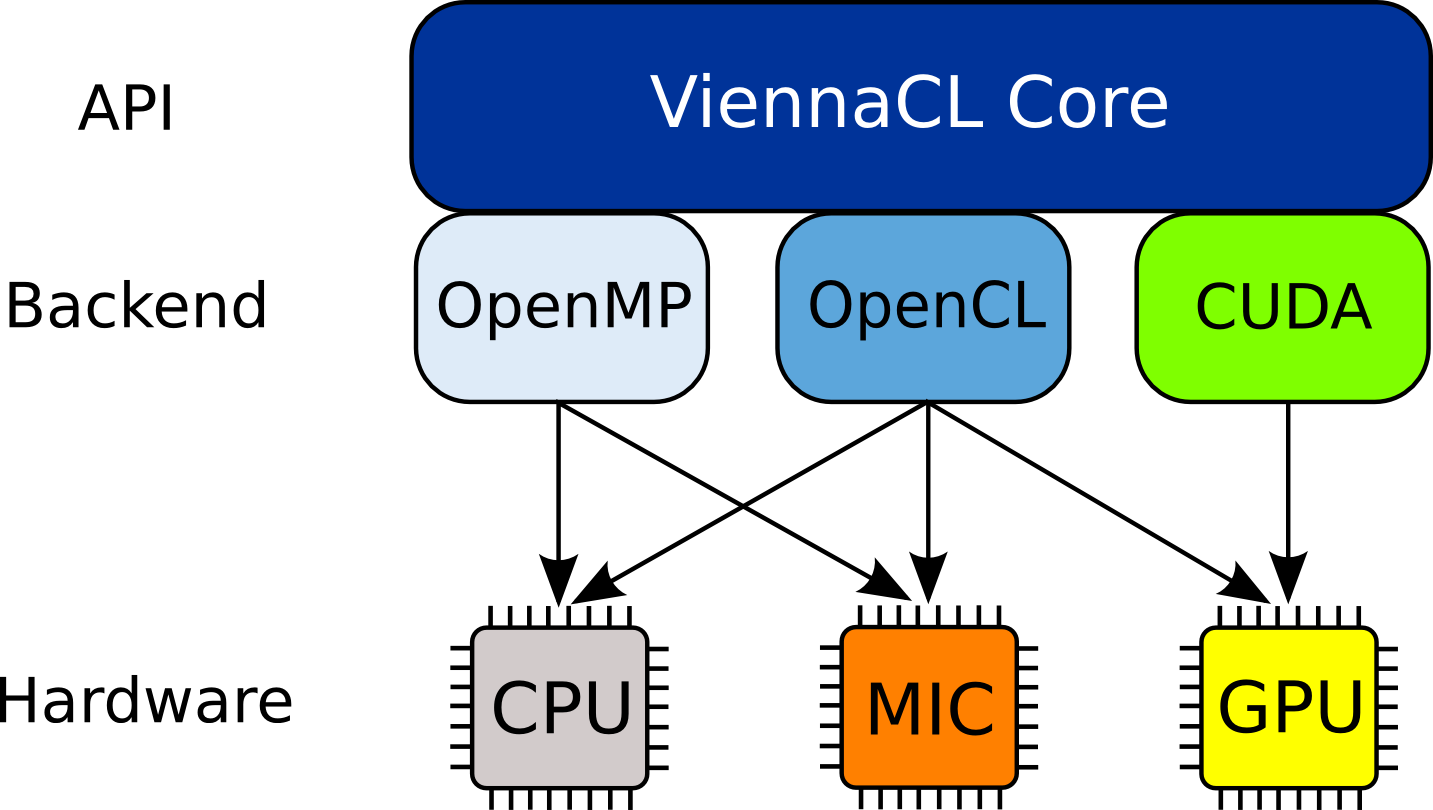
\includegraphics[width=0.999\textwidth]{figures/ViennaCL-arch}
\end{minipage}

  %\pause
  \vspace*{0.3cm}
  \begin{block}{Recent Advances}
  \begin{itemize}
   \item Pipelined Krylov solvers
   \item Fast sparse matrix-vector products
   \item Fast sparse matrix-matrix products
   \item Fine-grained algebraic multigrid
   \item Fine-grained parallel ILU
  \end{itemize}
  \end{block}

\end{frame}


\begin{frame}[fragile]
\frametitle{Current: PETSc + ViennaCL}

  \begin{block}{Current Use of ViennaCL in PETSc}
  \begin{itemize}
   \item 
  \begin{lstlisting}
 $> ./ex12 -vec_type viennacl -mat_type aijviennacl ...
  \end{lstlisting}
   \item Executes on OpenCL device
  \end{itemize}
  \end{block}

  %\pause
  
  \begin{block}{New Use of ViennaCL in PETSc}
  \begin{itemize}
   \item 
  \begin{lstlisting}
 $> ./ex12 -vec_type viennacl -mat_type aijviennacl
           -viennacl_backend openmp ...
  \end{lstlisting}
  \end{itemize}
  \end{block}

  %\pause
  
  \begin{block}{Pros and Cons}
  \begin{itemize}
   \item Use CPU + GPU simultaneously
   %\item Good PETSc performance on Theta, Aurora, Summit, ...
   \item Non-intrusive, use plugin-mechanism
   \item Non-optimal in strong-scaling limit
   \item Gather experiences for best long-term solution
  \end{itemize}
  \end{block}

\end{frame}





\begin{frame}{GPU Summary and Conclusion}

  \begin{block}{Currently Available}
    \begin{itemize}
     \item CUSP/CUDA for CUDA, ViennaCL for CUDA/OpenCL/OpenMP
     \item Automatic use for vector operations and SpMV
     \item Smoothed Agg. AMG via CUSP and ViennaCL
      \item ViennaCL as CUDA/OpenCL/OpenMP-hydra
    \end{itemize}
  \end{block}

  \begin{minipage}{0.7\textwidth}
    \begin{block}{Current Activities}
      \begin{itemize}
      \item GPU-acceleration for GAMG
      \item Better support for $n>1$ processes
      \item Use of cuBLAS and cuSPARSE
      \end{itemize}
    \end{block}
  \end{minipage}
  \begin{minipage}{0.29\textwidth}
    
\includegraphics[width=0.99\textwidth]{figures/hydra}
  \end{minipage}

\end{frame}


%%%% Conclusion




%
% Conclusion and Wrap-Up
%
\section{Conclusions}
\begin{frame}{Conclusions}
 
 \begin{block}{PETSc can help You}
  \begin{itemize}
   \item solve algebraic and DAE problems in your application area
   \item rapidly develop efficient parallel code, can start from examples
   \item develop new solution methods and data structures
   \item debug and analyze performance
   \item advice on software design, solution algorithms, and performance
   \item \centering \texttt{petsc-\{users,dev,maint\}@mcs.anl.gov}

  \end{itemize}
 \end{block}

 \begin{block}{You can help PETSc}
  \begin{itemize}
   \item report bugs and inconsistencies, or if you think there is a better way
   \item tell us if the documentation is inconsistent or unclear
   \item consider developing new algebraic methods as plugins, contribute if your idea works
  \end{itemize}
 \end{block}

\end{frame}


